% SOICT 2026 submission --- Track-B, v1 (2026-08-10) --- Springer LNCS format.
% Content = the finalized Track-B draft docs/paper/track_b_paper_draft.md: a single-basis nested
% ablation ladder P0 -> P1 -> P2 -> P3 -> G1 (P3 = G1 with the cross-stock graph disabled), classical
% econometric baselines, a multi-horizon graph null, and a parsimony finding. All numbers trace to the
% canonical result JSONs cited in the macro block below; keep the macros as the single source of truth.
% Template: llncs.cls from the official SOICT 2026 Springer template package.
% NOTE: verify llncs.cls/splncs04.bst against the official SOICT 2026 download before final submission.
%
\documentclass[runningheads]{llncs}
%
\usepackage[T1]{fontenc}
\usepackage{graphicx}
\usepackage{amsmath}
\usepackage{booktabs}
\usepackage{tikz}
\usetikzlibrary{arrows.meta,positioning,fit,backgrounds}
%
% ======================================================================
% Canonical number macros (single source of truth). All values are three-seed (42/123/2026) means
% unless noted. Source files:
%   ladder h5      : docs/reports/ladder_consistent_h5_2026-08-09_154402.json
%   multi-horizon  : docs/reports/ladder_consistent_h{1,10,22}_2026-08-09_180326.json (+ _multihorizon .md)
%   classical      : docs/reports/classical_baselines_h5_2026-08-10_221043.json
% ----------------------------------------------------------------------
% Proposed model G1 --- held-out TEST (h5).
\newcommand{\GtestQ}{0.5759}     % QLIKE (raw 0.575926)
\newcommand{\GtestR}{0.002305}   % RMSE  (raw 0.00230527)
\newcommand{\GtestM}{0.0005996}  % MAE   (raw 0.000599607)
\newcommand{\GtestRsq}{0.7635}   % R^2   (raw 0.763520)
\newcommand{\GtestD}{48.22}      % DirAcc% (raw 48.221)
% Proposed model G1 --- VAL (h5).
\newcommand{\GvalQ}{0.5091}      % QLIKE (raw 0.509102)
% Backbone rungs --- TEST QLIKE (h5).
\newcommand{\PzeroTestQ}{0.5676} % P0 HAR-linear (raw 0.567625)
\newcommand{\PoneTestQ}{0.5648}  % P1 price LSTM (raw 0.564780)
\newcommand{\PtwoTestQ}{0.5599}  % P2 +news      (raw 0.559854)  <-- best test QLIKE in study
\newcommand{\PthreeTestQ}{0.5765}% P3 +gate      (raw 0.576488)
% Backbone rungs --- VAL QLIKE (h5).
\newcommand{\PoneValQ}{0.5062}   % P1 (raw 0.506196)
\newcommand{\PtwoValQ}{0.5031}   % P2 (raw 0.503117)  <-- best val QLIKE among backbone
\newcommand{\PthreeValQ}{0.5130} % P3 (raw 0.513001)
% Classical econometric baselines --- TEST (h5).
\newcommand{\HARtestQ}{0.5793}   % HAR   QLIKE (raw 0.579291)
\newcommand{\HARtestRsq}{0.7667} % HAR   R^2   (raw 0.766703)
\newcommand{\HARQtestQ}{0.5737}  % HARQ  QLIKE (raw 0.573674)  <-- best classical test QLIKE
\newcommand{\HARQtestRsq}{0.7668}% HARQ  R^2   (raw 0.766817)
\newcommand{\EWMAtestQ}{0.6006}  % EWMA  QLIKE (raw 0.600625)
\newcommand{\GARCHtestQ}{1.7514} % GARCH QLIKE (raw 1.75138)
\newcommand{\GARCHtestRsq}{0.0031}% GARCH R^2  (raw 0.003075)
% Graph ablation G1 vs P3 (exactly nested; graph-off determinism 0.0).
\newcommand{\graphTestP}{0.79}   % TEST paired-t p over seeds (raw 0.7913)
\newcommand{\graphValP}{0.010}   % VAL  paired-t p over seeds (raw 0.0096)
% News ablation P2 vs P1 paired-t (QLIKE), from per-seed ladder entries.
\newcommand{\newsValT}{-7.69}
\newcommand{\newsTestT}{-9.50}
% Gate ablation P3 vs P2 paired-t (QLIKE), from per-seed ladder entries.
\newcommand{\gateTestT}{+35.8}
% Observation counts and constants.
\newcommand{\nval}{14{,}418}
\newcommand{\ntest}{14{,}464}
\newcommand{\tcrit}{4.30}
\newcommand{\nseed}{3}
\newcommand{\ntick}{33}
%
\begin{document}
%
\title{A News-Augmented Cross-Stock Graph LSTM for VN30 Volatility Forecasting: A Component Ablation from HAR to Masked Message-Passing}
%
\titlerunning{News-Augmented Cross-Stock Graph LSTM for VN30 Volatility}
%
\author{Author One\inst{1} \and Author Two\inst{1}}
\authorrunning{Author One et al.}
%
\institute{VNUHCM University of Science, Ho Chi Minh City, Vietnam\\
\email{\{author1,author2\}@student.hcmus.edu.vn}}
%
\maketitle
%
\begin{abstract}
Volatility forecasts set risk limits, margin, and option prices for VN30, the most liquid stocks on
Vietnam's Ho Chi Minh Stock Exchange. Price-only forecasters ignore the Vietnamese-language news that
plausibly signals volatility shocks, and mature-market cross-stock graph models do not transfer to an
emerging market whose listing calendars are sparse and unbalanced. We propose a pooled news-augmented
cross-stock graph LSTM (G1) for five-day-ahead VN30 volatility. Each ticker-day is one asynchronous
sample, which recovers the full trading calendar rather than the 26\% synchronized-date intersection a
fixed-node graph would require. G1 combines a shared temporal LSTM over the three HAR volatility scales,
a PhoBERT news branch, a per-ticker news gate, and a cross-stock message-passing layer over an
availability-aware masked adjacency. We evaluate G1 with a single-basis nested ablation ladder,
$\text{P0 (HAR)}\to\text{P1 (price LSTM)}\to\text{P2 (+news)}\to\text{P3 (+gate)}\to\text{G1 (+graph)}$,
where P3 is exactly G1 with the message-passing residual disabled (graph-off readout determinism $0.0$).
All rungs and seven classical econometric baselines score on the same \nval{} validation and \ntest{}
test observations. News content carries the forecast gain: adding the news branch lowers QLIKE
significantly on validation ($t=\newsValT$) and held-out test ($t=\newsTestT$), and the parsimonious
news backbone (P2) attains the lowest test QLIKE in the study (\PtwoTestQ). The per-ticker gate raises
QLIKE and earns no place. Enabling the cross-stock graph (G1 vs P3) yields no statistically significant
QLIKE improvement at any of four horizons under a Diebold--Mariano test (verdict B, graph null). A
targeted sweep confirms this: neither the base graph nor five research-backed enhancements (QLIKE-loss
training, HAR $+$ graph-residual, directed spillover edges, learned adjacency, omit-self-loop) beats a
well-specified HAR at a Diebold--Mariano-significant level. HAR and
HARQ tie the deep models on the level metrics (test QLIKE \HARtestQ{} and \HARQtestQ, $R^2\approx0.767$),
while GARCH-family models are far worse (test QLIKE $1.75$--$1.86$, $R^2\approx0$). We present G1 as the
proposed architecture and report a rigorous parsimony finding: news content improves the forecast but
cross-stock graph propagation does not. Directional accuracy stays near $48\%$ for every forecaster
because the daily Parkinson target's day-to-day change is anti-persistent (sign lag-1 autocorrelation
$-0.30$, negative for all \ntick{} tickers).

\keywords{Volatility forecasting \and Graph neural networks \and Financial news \and PhoBERT \and
Pooled panel \and Emerging markets.}
\end{abstract}
%
% ======================================================================
\section{Introduction}
\label{sec:intro}
Volatility forecasts drive the daily risk decisions of every desk that trades VN30, the basket of
roughly thirty most liquid stocks on Vietnam's Ho Chi Minh Stock Exchange. A margin engine sizes
collateral from forecast volatility; an option desk prices from it; a risk officer sets position limits
against it. When the forecast tracks tomorrow's realized volatility poorly, each decision pays for the
error. VN30 desks make these decisions inside an information environment that a price-only forecaster
discards: a steady flow of Vietnamese-language news that plausibly signals volatility shocks before they
reach the price range, and a web of cross-stock spillovers a univariate model cannot represent.

The classical Heterogeneous Autoregressive (HAR) model of Corsi~\cite{corsi2009}, the linear univariate
workhorse that regresses future volatility on its own daily, weekly, and monthly averages, admits
neither signal. Two structural extensions could close the gap: a news channel that reads text, and a
cross-stock graph. Recent financial graph neural networks add cross-stock
coupling~\cite{velickovic2018,chen2022,zhang2025gnnhar}, but they operate on large, long-lived,
calendar-synchronized markets. VN30 is different. Its listing dates are severely unbalanced: the newest
constituent (SSB, listed 2021) trades on about 1{,}300 sessions while the oldest (VNM, ACB) trade on
about 4{,}900. A fixed cross-stock graph over \ntick{} nodes needs every node present on the same
trading date, which keeps only about 1{,}296 dates, roughly 26\% of the 4{,}989-date union, and starves
the graph model before it trains. Whether cross-stock structure helps VN30 volatility is therefore an
open question the standard fixed-node design cannot answer without confounding graph signal with data
scarcity.

We resolve the confound by pooling every ticker-day as one asynchronous sample, which recovers the full
timeline, and by running the graph on an availability-aware masked adjacency that builds edges per date
over only the tickers present that day. On this foundation we propose a news-augmented cross-stock graph
LSTM (G1) with four components, and evaluate it with a nested ablation that removes one part at a time
down to the classical HAR baseline, grounded against seven classical econometric baselines on the
identical observation set. This paper makes four contributions.
\begin{enumerate}
\item \textbf{A pooled news-augmented cross-stock graph LSTM (G1).} The architecture combines temporal,
textual, and cross-stock structure on a pooled asynchronous panel, and its graph runs on an
availability-aware masked adjacency that recovers the full 4{,}989-date union without imputing
pre-listing history (Section~\ref{sec:method}). The masked cross-stock formulation is the architectural
novelty for a sparse emerging-market panel.
\item \textbf{A single-basis nested ablation from the full model to the classical HAR baseline.}
Removing the message-passing residual from G1 lands exactly on P3 (graph-off determinism $0.0$); removing
the gate, the news branch, and temporal learning in turn reaches HAR. All rungs score on the same \nval{}
validation and \ntest{} test observations, so each step is one controlled increment
(Section~\ref{sec:results}).
\item \textbf{News content earns its place; the gate and the cross-stock graph do not.} News lowers QLIKE
significantly on validation and held-out test; the gate raises QLIKE; enabling the graph gives no
statistically significant QLIKE improvement under a Diebold--Mariano test at any of four horizons.
Classical HAR-family models tie the deep models while GARCH is far worse. We report a rigorous parsimony
finding (Sections~\ref{sec:results} and~\ref{sec:discussion}).
\item \textbf{Direction is near-random by construction.} No model reaches $49\%$ directional accuracy,
and model-free forecasters reach the same ceiling, because the daily Parkinson target's day-to-day change
is anti-persistent (Sections~\ref{sec:results} and~\ref{sec:discussion}).
\end{enumerate}

% ======================================================================
\section{Background and Problem Setup}
\label{sec:background}

\subsubsection{Parkinson volatility.}
We forecast daily volatility measured by the Parkinson range estimator, which uses the intraday high $H$
and low $L$:
\begin{equation}
\sigma^2_{\text{Park}} = \frac{\left(\ln(H/L)\right)^2}{4\ln 2}.
\label{eq:parkinson}
\end{equation}
The range estimator uses more of the day's price path than a close-to-close estimator and is a standard
choice for daily data~\cite{parkinson1980}. Every model in this paper, deep and classical, forecasts the
same daily realized-variance quantity. It is a noisy one-day proxy for latent volatility, a fact
Section~\ref{sec:discussion} shows matters for the direction task.

\subsubsection{The HAR decomposition and baseline.}
The HAR model~\cite{corsi2009} predicts future volatility from three moving averages of past volatility,
over daily (1-day), weekly (5-day), and monthly (22-day) windows, approximating volatility's long memory
with a parsimonious linear regression, and remains the benchmark a new daily-volatility forecaster must
beat. The HARQ extension~\cite{bpq2016} shrinks the daily coefficient when the volatility estimate is
noisy. We use the three HAR averages both as the input of the temporal branch and, as a plain linear
regression, as the classical HAR baseline (P0).

\subsubsection{Forecast target and losses.}
For each stock and day $t$ we predict the Parkinson volatility five trading days ahead, a single-day
value at $t+5$. We train with mean squared error on normalized targets and evaluate on the raw scale with
six metrics: MSE, RMSE, MAE, $R^2$, QLIKE, and directional accuracy. QLIKE, the quasi-likelihood loss
standard in the realized-volatility literature~\cite{patton2011}, penalizes under-prediction more than
over-prediction and tolerates the noise in the volatility proxy:
\begin{equation}
\text{QLIKE} = \frac{1}{T}\sum_{t=1}^{T}\left(\frac{\hat{\sigma}^2_t}{\sigma^2_t}
 - \ln\frac{\hat{\sigma}^2_t}{\sigma^2_t} - 1\right).
\label{eq:qlike}
\end{equation}
Directional accuracy compares $\operatorname{sign}(\hat{y}_{i,t+1}-\hat{y}_{i,t})$ against
$\operatorname{sign}(y_{i,t+1}-y_{i,t})$ per ticker over time, then averages across tickers, so a
difference never crosses a ticker boundary.

% ======================================================================
\section{Method}
\label{sec:method}
We describe the proposed model G1 first, then define the ablation ladder as component removals from it.
G1 forecasts one ticker's five-day-ahead volatility from four inputs: a 22-day price window of the three
HAR scales, a 22-day news window of PhoBERT features with a mask, the ticker identity, and the set of
other tickers trading on the same date. All encoders share weights across tickers.

\begin{figure}[t]
\centering
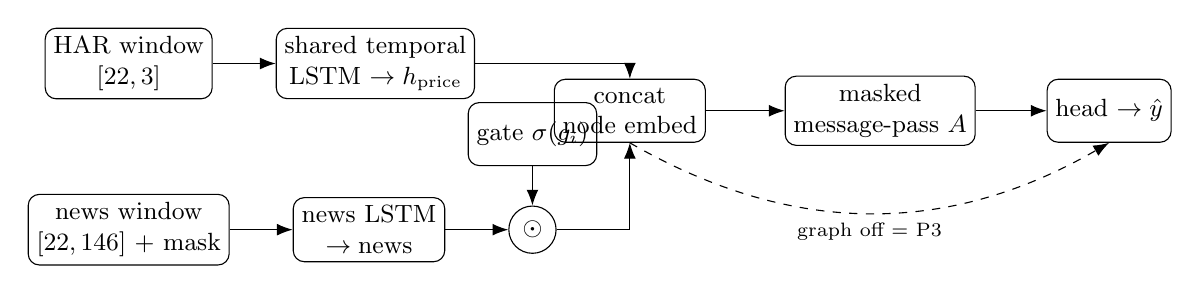
\begin{tikzpicture}[
  font=\small,
  box/.style={draw, rounded corners, align=center, minimum height=8mm, inner sep=3pt},
  op/.style={draw, circle, inner sep=1pt, minimum size=6mm},
  >={Latex[length=2mm]}
]
\node[box] (harin) {HAR window\\ $[22,3]$};
\node[box, right=8mm of harin] (lstm) {shared temporal\\ LSTM $\to h_{\text{price}}$};
\node[box, below=12mm of harin] (newsin) {news window\\ $[22,146]$ + mask};
\node[box, right=8mm of newsin] (newslstm) {news LSTM\\ $\to \text{news}$};
\node[op, right=8mm of newslstm] (mult) {$\odot$};
\node[box, above=5mm of mult] (gate) {gate $\sigma(g_i)$};
\node[box, right=10mm of lstm, yshift=-6mm] (concat) {concat\\ node embed};
\node[box, right=10mm of concat] (mp) {masked\\ message-pass $A$};
\node[box, right=9mm of mp] (head) {head $\to \hat{y}$};
\draw[->] (harin) -- (lstm);
\draw[->] (newsin) -- (newslstm);
\draw[->] (newslstm) -- (mult);
\draw[->] (gate) -- (mult);
\draw[->] (lstm) -| (concat);
\draw[->] (mult) -| (concat);
\draw[->] (concat) -- (mp);
\draw[->] (mp) -- (head);
\draw[->,dashed] (concat.south) to[out=-30,in=-150] node[below,font=\scriptsize]{graph off $=$ P3} (head.south);
\end{tikzpicture}
\caption{The proposed model G1. A shared temporal LSTM encodes the HAR window; a news LSTM encodes
PhoBERT features scaled by a per-ticker gate $\sigma(g_i)$; the concatenated node embedding passes through
a residual cross-stock message-passing layer over the availability-aware masked adjacency $A$, then a
shared head. Disabling the message-passing residual (dashed path) gives exactly P3.}
\label{fig:arch}
\end{figure}

\subsection{The proposed model G1}
Four components combine in sequence (Fig.~\ref{fig:arch}). (i)~A shared two-layer temporal LSTM (hidden
size 64, dropout 0.2) reads each ticker's HAR window into a price representation. (ii)~A shared news
encoder maps the 146-dimensional daily news vector through a linear-plus-ReLU layer into a single-layer
LSTM (hidden size 64) over the window; the mask lets an all-missing window yield a finite vector.
(iii)~A per-ticker gate scales the news representation by a learned scalar per stock,
\begin{equation}
\text{news}^{\text{gated}}_{i} = \sigma(g_i)\cdot \text{news}_{i}, \qquad i=1,\dots,N,
\label{eq:gate}
\end{equation}
so the model admits a stock-specific amount of news; the gated news and the price representation
concatenate into a per-node embedding. (iv)~A residual cross-stock message-passing layer shares
information between stocks, $\text{base}\leftarrow\text{base}+\text{MP}(\text{base},A,\text{mask})$, where
$A$ is an availability-aware adjacency built per date over the present tickers and the mask restricts
aggregation to present neighbours. A shared head maps the propagated embedding to the forecast. The
masked cross-stock message-passing is the architectural novelty.

\subsection{Availability-aware masked adjacency}
Rather than intersecting to synchronized dates, we build the adjacency per date over the present tickers
and mask absent nodes and edges. This recovers the union timeline, and the masked evaluation sets contain
exactly the same present-node observations as the ladder backbone, which makes the graph on/off comparison
fair. The headline adjacency is $k$-nearest-neighbour with $k=8$ (average $5.87$ off-diagonal edges per
present row). A positivity floor clamps denormalized predictions away from non-positive volatility before
QLIKE (non-positive-prediction rate $0.0$ on the masked manifest).

\subsection{The nested ablation ladder}
The ladder removes one component of G1 at a time, and every rung scores on the identical observation set.
\begin{itemize}
\item \textbf{G1 (full model):} all four components.
\item \textbf{P3 (remove the cross-stock graph):} G1 with the message-passing residual disabled. P3 is
\emph{exactly} G1 with the graph switched off---removing the residual lands on P3 with a graph-off readout
determinism of $0.0$ for every seed and horizon, so the G1-versus-P3 pair is the clean, exactly-nested
control that isolates cross-stock propagation. There is no separate graph-off row.
\item \textbf{P2 (remove the per-ticker gate):} the news-augmented backbone without the gate.
\item \textbf{P1 (remove the news branch):} a price-only LSTM.
\item \textbf{P0 (remove temporal learning):} a closed-form per-ticker linear regression on the three HAR
averages---the classical HAR baseline.
\end{itemize}
G1 is trained end-to-end; P3 is G1 read out with the message-passing disabled, so it shares G1's weights
exactly. The ladder is therefore one consistent basis, not two separately trained families.

% ======================================================================
\section{Experimental Setup}
\label{sec:setup}

\subsubsection{Universe, split, and leakage control.}
We use \ntick{} VN30 constituents with daily OHLCV data; series lengths range from about 1{,}300 sessions
(SSB) to about 4{,}900 (VNM, ACB). We exclude two short-history current members (BSR, VPL). We split each
series chronologically into 70\% train, 15\% validation, 15\% test before generating HAR features, fitting
scalers, or building windows. Per-ticker scalers are fit on the training partition only and selected by
explicit ticker id; the graph adjacency is graph-bound to the training window. A news feature uses only
information available by the sample's forecast origin (15:00 Asia/Ho\_Chi\_Minh on the final input date).
On the masked five-day manifest the evaluation sets hold \nval{} present-node validation and \ntest{} test
observations, shared across every rung and baseline; the graph runs over $6{,}470$ per-date snapshots.

\subsubsection{Training objective and hyperparameters.}
All deep configurations minimize mean squared error on per-ticker normalized targets; QLIKE and the other
metrics are computed only at evaluation on the raw scale, so the proportional loss never enters the
gradient. Optimization uses Adam (learning rate $10^{-3}$, weight decay $10^{-5}$), dropout $0.2$, and
gradient-norm clipping at $1.0$, with best-validation checkpoint selection; each window is 22 trading days
and the horizon is five. P0 is a closed-form least-squares fit. Every run seeds Python, NumPy, and Torch
(including CUDA); the three seeds 42/123/2026 are independent repetitions. Switching the training loss to
QLIKE is a lever the literature identifies as decisive for beating HAR~\cite{zhang2025gnnhar}; we keep MSE
training here so the ablation isolates architecture rather than objective, and flag QLIKE training as
future work.

\subsubsection{Significance.}
With three seeds the two-sided 5\% paired-$t$ threshold at two degrees of freedom is $|t|>\tcrit$. We
complement the paired-$t$ with a Diebold--Mariano (DM) test on the per-observation QLIKE and MSE loss
series (HAC truncation lag $h-1$, Harvey--Leybourne--Newbold corrected). We attempted a Model Confidence
Set over the ladder and classical baselines, but the result artifacts store per-configuration metrics
rather than per-observation prediction series, and clean re-scoring onto a single common observation set
was not feasible within the submission window, so the DM tests are the
primary graph-significance evidence.

\subsubsection{Classical baselines.}
On the identical val/test keys and raw targets, scored by the same routine as the deep ladder, we fit a
persistence forecast, an EWMA, the classical HAR, a HARQ variant with a daily range-based
realized-quarticity proxy (the canonical 5-minute quarticity is not identified on daily OHLCV), a log-HAR,
and GARCH(1,1), GJR-GARCH, and EGARCH per ticker on close-to-close log returns. The GARCH family covers all
\ntick{} tickers on the full observation set: LPB's raw OHLCV was recovered from the SSI iBoard API (SSI's
different price-adjustment convention is immaterial for return-based GARCH, and 18 LPB holiday dates absent
from the SSI trading calendar use the carried-forward forecast from the last trading origin).
All models were run in PyTorch on an NVIDIA GeForce RTX~4060 Laptop GPU under PyTorch~2.6 with CUDA~12.4.

% ======================================================================
\section{Results}
\label{sec:results}
Every rung and baseline scores on the same \nval{} validation / \ntest{} test observations, so all levels
are directly comparable.

\subsection{The proposed model versus classical econometric baselines}
\label{sec:baselines}
Table~\ref{tab:classical} places G1 against the classical baselines on the held-out test split. G1 reaches
test QLIKE~\GtestQ{} and $R^2$~\GtestRsq. The classical HAR reaches QLIKE~\HARtestQ{} and HARQ~\HARQtestQ{}
at $R^2\approx0.767$; EWMA reaches~\EWMAtestQ. On the level metrics the HAR family and the deep models tie:
HARQ's test QLIKE is marginally below G1's, and G1's $R^2$ is within $0.004$ of HAR's. The GARCH family is
far worse on every level metric (test QLIKE~\GARCHtestQ{}--$1.86$, $R^2$ from~\GARCHtestRsq{} to $-0.003$),
and the persistence forecast collapses on QLIKE. The headline is a tie between the deep news-augmented
system and the field-standard HAR/HARQ, and a decisive win of both over GARCH.

\begin{table}[t]
\caption{Five-day-ahead held-out test metrics: proposed model G1 and classical econometric baselines. Same
\ntest{} observations for all rows including the GARCH family (33/33 tickers). Deep rows are \nseed-seed means;
classical rows are single deterministic fits. Lower is better for QLIKE, RMSE, MAE; higher for $R^2$,
DirAcc. Bold marks the best value per column. Source:
\texttt{ladder\_consistent\_h5} and \texttt{classical\_baselines\_h5}.}
\label{tab:classical}
\centering
\begin{tabular}{lccccc}
\toprule
Model & QLIKE & RMSE & $R^2$ & DirAcc (\%) \\
\midrule
G1 (proposed)     & $0.5759$          & $0.002305$          & $0.7635$          & $48.22$ \\
HAR               & $0.5793$          & $0.002290$          & $0.7667$          & $48.40$ \\
HARQ              & $\mathbf{0.5737}$ & $\mathbf{0.002289}$ & $\mathbf{0.7668}$ & $48.38$ \\
log-HAR           & $0.7794$          & $0.002372$          & $0.7496$          & $\mathbf{48.83}$ \\
EWMA              & $0.6006$          & $0.002311$          & $0.7624$          & $48.03$ \\
Persistence       & $4151.2$          & $0.002772$          & $0.6580$          & $48.01$ \\
GARCH(1,1)        & $1.7514$          & $0.004733$          & $0.0034$          & $48.49$ \\
GJR-GARCH         & $1.8141$          & $0.004738$          & $0.0010$          & $48.40$ \\
EGARCH            & $1.8633$          & $0.004747$          & $-0.0029$         & $48.64$ \\
\bottomrule
\end{tabular}
\end{table}

\subsection{The nested ladder: news is decisive, the gate does not pay its way}
\label{sec:ladder}
Table~\ref{tab:ladder} reports the full ladder, validation and test, \nseed-seed mean. The price-only LSTM
(P1) lowers test RMSE against HAR-linear P0 and lowers QLIKE on both splits, so temporal learning already
buys a proportional-loss gain. Adding news (P2) is the decisive step: it lowers validation QLIKE from
\PoneValQ{} to \PtwoValQ{} and test QLIKE from \PoneTestQ{} to \PtwoTestQ. P2---the parsimonious
news-augmented backbone with neither gate nor graph---attains the lowest test QLIKE of any configuration
in the study, below HARQ's~\HARQtestQ. Adding the gate (P3) does not extend the gain: its test QLIKE
(\PthreeTestQ) is above P2's. Table~\ref{tab:pairedt} gives paired-$t$ tests derived from the per-seed
ladder entries. Adding news lowers QLIKE significantly on both splits ($t=\newsValT$ validation,
$t=\newsTestT$ test); on validation it also improves MSE, RMSE, and $R^2$, while on test it trades a small
significant increase in squared error for the QLIKE and MAE gain. Adding the gate does not lower QLIKE---it
raises it significantly ($t=\gateTestT$ on test).

\begin{table}[t]
\caption{Five-day-ahead ladder metrics, validation and test, \nseed-seed mean (42/123/2026). Same \nval{}
validation / \ntest{} test observations across rows. Bold marks the best value per column within each
split. Source: \texttt{ladder\_consistent\_h5}.}
\label{tab:ladder}
\centering
\begin{tabular}{llccccc}
\toprule
Split & Config & RMSE & MAE & $R^2$ & QLIKE & DirAcc (\%) \\
\midrule
VAL  & P0 HAR         & $0.001472$          & $0.0004737$          & $0.7394$          & $0.5096$          & $48.52$ \\
VAL  & P1 price LSTM  & $0.001492$          & $0.0004859$          & $0.7324$          & $0.5062$          & $48.54$ \\
VAL  & P2 +news       & $0.001479$          & $0.0004763$          & $0.7371$          & $\mathbf{0.5031}$ & $48.52$ \\
VAL  & P3 +gate       & $0.001468$          & $0.0004668$          & $0.7410$          & $0.5130$          & $48.44$ \\
VAL  & G1 +graph      & $\mathbf{0.001455}$ & $\mathbf{0.0004619}$ & $\mathbf{0.7454}$ & $0.5091$          & $\mathbf{48.68}$ \\
\midrule
TEST & P0 HAR         & $0.002289$          & $0.0006027$          & $0.7668$          & $0.5676$          & $\mathbf{48.53}$ \\
TEST & P1 price LSTM  & $\mathbf{0.002265}$ & $0.0006065$          & $\mathbf{0.7718}$ & $0.5648$          & $47.98$ \\
TEST & P2 +news       & $0.002270$          & $0.0006016$          & $0.7706$          & $\mathbf{0.5599}$ & $48.04$ \\
TEST & P3 +gate       & $0.002313$          & $0.0006014$          & $0.7620$          & $0.5765$          & $47.88$ \\
TEST & G1 +graph      & $0.002305$          & $\mathbf{0.0005996}$ & $0.7635$          & $0.5759$          & $48.22$ \\
\bottomrule
\end{tabular}
\end{table}

\begin{table}[t]
\caption{Paired-$t$ tests across three seeds (df=2, threshold $|t|>\tcrit$), derived from the per-seed
entries of the ladder JSON. Sign is (upper rung $-$ lower rung); negative $t$ on QLIKE means the added
component lowers QLIKE. Source: \texttt{ladder\_consistent\_h5} (per-seed values).}
\label{tab:pairedt}
\centering
\begin{tabular}{llccccc}
\toprule
Contrast & Split & MSE & RMSE & $R^2$ & QLIKE \\
\midrule
News (P2 vs P1) & VAL  & $-4.38$ (sig.) & $-4.38$ (sig.) & $+4.38$ (sig.) & $-7.69$ (sig.) \\
News (P2 vs P1) & TEST & $+10.6$ (worse) & $+10.7$ (worse) & $-10.6$ (worse) & $-9.50$ (sig.) \\
Gate (P3 vs P2) & VAL  & $-7.32$ & $-7.37$ & $+7.32$ & $+30.6$ (worse) \\
Gate (P3 vs P2) & TEST & $+27.6$ (worse) & $+28.4$ (worse) & $-27.6$ (worse) & $+35.8$ (worse) \\
LSTM (P1 vs P0) & VAL  & $+9.17$ (worse) & $+9.24$ (worse) & $-9.17$ (worse) & $-6.09$ (sig.) \\
LSTM (P1 vs P0) & TEST & $-25.7$ (better) & $-25.6$ (better) & $+25.7$ (better) & $-3.83$ (n.s.) \\
\bottomrule
\end{tabular}
\end{table}

\subsection{Graph ablation: removing cross-stock message-passing changes nothing significant}
\label{sec:graph}
Table~\ref{tab:graph} isolates the cross-stock graph by the exactly-nested G1-versus-P3 pair. Because P3
is G1 read out with the residual disabled (determinism $0.0$), the pair differs only in cross-stock
propagation. On validation the graph lowers loss on all three seeds (paired-$t$ $p=\graphValP$), but the
per-observation DM test on QLIKE is not significant-negative on all seeds, so the validation verdict is B.
On the held-out test the case disappears: G1's QLIKE (\GtestQ) improves on P3's (\PthreeTestQ) by less than
its fourth significant figure, holds on only two of three seeds, and the paired-$t$ is not significant
($p=\graphTestP$).

\begin{table}[t]
\caption{Multi-horizon graph ablation G1 vs P3 (exactly nested), held-out test, \nseed-seed mean. QLIKE
$\Delta=$ mean(G1 $-$ P3) over seeds (negative $=$ graph helps); paired-$t$ $p$ across seeds. Verdict B $=$
graph null (G1 not below P3 on QLIKE in all seeds AND per-seed DM-QLIKE not significant-negative in all
seeds). Source: \texttt{ladder\_consistent\_h\{1,5,10,22\}} and \texttt{\_multihorizon}.}
\label{tab:graph}
\centering
\begin{tabular}{cccccc}
\toprule
Horizon & TEST P3 QLIKE & TEST G1 QLIKE & QLIKE $\Delta$ & test paired-$t$ $p$ & Verdict \\
\midrule
1  & $0.4857$ & $0.5166$ & $+0.0309$  & $0.531$ & B (null) \\
5  & $0.5765$ & $0.5759$ & $-0.00056$ & $0.791$ & B (null) \\
10 & $0.6168$ & $0.6156$ & $-0.0012$  & $0.067$ & B (null) \\
22 & $0.6738$ & $0.6787$ & $+0.0049$  & $0.143$ & B (null) \\
\bottomrule
\end{tabular}
\end{table}

\subsection{The null holds across all four horizons}
\label{sec:multihorizon}
Table~\ref{tab:graph} replicates the exactly-nested graph ablation at horizons 1, 5, 10, and 22 trading
days, each on its own leakage-safe masked manifest. The verdict is B (graph null) at every horizon. Two
nuances are worth stating plainly. At h1 the graph does improve the squared-error metrics---DM on the MSE
loss series is significant-negative on all three test seeds---but its QLIKE is unstable: seed 2026 inflates
G1's QLIKE through near-floor one-day predictions (the val G1 QLIKE outlier of $0.878$), so the
QLIKE-based verdict stays B. At h22 the graph improves validation QLIKE (paired-$t$ $p=0.0002$) but the
gain does not carry to the held-out test, where G1 is worse than P3 on all three seeds. h5 and h10 are the
cleanest nulls. Across all four horizons the graph does not deliver a statistically significant QLIKE
improvement over the news-augmented backbone.

\subsection{Direction is near-random for every model}
\label{sec:direction}
Directional accuracy sits at $47.9\%$--$48.7\%$ across the ladder and $48.0\%$--$48.8\%$ across the
classical baselines, at or below the $50\%$ no-skill line. No paired test separates any configuration on
direction, and the model-free persistence and EWMA forecasters reach the same band.
Section~\ref{sec:discussion} explains why.

% ======================================================================
\section{Discussion}
\label{sec:discussion}

\subsubsection{What each component contributes.}
The single-basis ladder gives a clean attribution. Temporal learning (P1) buys a proportional-loss gain
over HAR. News content (P2) is decisive: it lowers QLIKE significantly on validation and held-out test,
and the parsimonious P2 backbone attains the lowest test QLIKE of any model in the study. The per-ticker
gate (P3) does not extend the gain and raises QLIKE. The cross-stock graph (G1 vs P3) yields no
statistically significant QLIKE improvement at any of four horizons. Only temporal learning and news
content carry a measurable forecast gain on this panel.

\subsubsection{Why the graph adds nothing, and why the null is clean.}
Three facts bound the graph contribution. First, the message-passing layer aggregates news that has
already entered each node's own representation, so the marginal information a neighbour adds on a daily
panel is small. Second, VN30's listing-date imbalance thins the early-year neighbourhoods even under
masking. Third, the masked formulation removes the data-volume confound a synchronized-intersection graph
would suffer, and the exact nesting (P3 is G1 with the graph off, determinism $0.0$) removes any
training-setup confound, so the null speaks to the cross-stock signal itself. It replicates across four
horizons and under a DM test. It aligns with the best-controlled published GNN-vs-HAR study, GNNHAR on
DJIA-30, where multi-hop graph spillover gave no clear advantage under a Model Confidence Set and the
gains came from nonlinearity and a QLIKE loss, not the graph~\cite{zhang2025gnnhar}, and with the broader
finding that a well-specified HAR is hard to beat on a limited information set~\cite{audrino2025}.

\subsubsection{Classical baselines confirm the ceiling.}
HAR and HARQ tie the deep models on the level metrics (test QLIKE~\HARtestQ/\HARQtestQ, $R^2\approx0.767$),
and HARQ's QLIKE is marginally below G1's, while the GARCH family is far worse. A well-specified HAR-family
model sits near a structural ceiling for daily range-based variance on a small universe, so the deep
model's value is that it matches HAR while adding a news channel, not that it dominates HAR on the level.

\subsubsection{Attempts to strengthen the graph and future directions.}
The published record indicates the levers that separate a graph that beats HAR from one that ties it, most
of which this regime lacks: intraday-derived realized variance, a QLIKE training loss, directed
volatility-spillover edges, richer HAR-family node features (semivariance, realized-quarticity, overnight
and range estimators), and a large cross-sectional universe~\cite{zhang2025gnnhar,audrino2025,bpq2016}. The
three realistic on-data levers are (i)~a QLIKE training objective, (ii)~range-estimator, overnight, and
HAR-residual node features, and (iii)~a directed Diebold--Yilmaz spillover adjacency in place of
correlation $k$-NN. We ran that targeted sweep on the identical consistent basis (same \nval{}
validation / \ntest{} test observations, leakage-safe masked $k$-NN-8 graph, three seeds), evaluating a
leaner price-only GAT and five research-backed levers against the pooled-HAR anchor P0 (test QLIKE
$0.5676$): (C1)~a QLIKE-loss GAT on the news backbone, (C2)~an additive HAR $+$ graph-residual
decomposition, (C3)~directed Diebold--Yilmaz volatility-spillover edges, (C5)~spillover with an omitted
self-loop under a $k$-sweep, and (C6)~a learned dynamic adjacency. No configuration beats the anchor at a
Diebold--Mariano-significant level on QLIKE. The best, C2, reaches test QLIKE $0.5662$ but its per-seed
sign is inconsistent and the across-seed paired-$t$ is far from significant ($p=0.562$), so it
statistically ties P0 rather than beating it, and ties P0 on RMSE. The QLIKE-loss GAT (C1, test QLIKE
$0.5730$) improves on the MSE-trained backbone and beats the classical per-ticker HAR ($0.5793$) and ties
P0 on RMSE, but is significantly worse than the pooled-HAR anchor on QLIKE (paired-$t$ $p=0.027$). The
directed-spillover, omit-self, and learned-adjacency variants (C3 $0.5908$, C5 $0.5748$, C6 $0.5903$) are
significantly worse than P0 on QLIKE. A separate leaner check, a price-only GAT on the P1 backbone, beats
HAR on only one of six held-out test metrics (MAE) and is directionally, though not significantly, worse
on squared-error loss (Diebold--Mariano $p=0.19$--$0.25$). Two further levers were not run: HAR-RV-X
range/overnight node features (C4) need a multi-feature backbone beyond the pooled preprocessor's
single-feature contract, and news-as-edge co-mention (C7) is infeasible on the per-ticker news panel.
Neither the base graph nor any of the five targeted enhancements beats a well-specified HAR, which
strengthens rather than weakens the parsimony conclusion: the cross-stock graph adds no measurable value
even under the levers the literature credits for closing the HAR gap.
% Sweep numbers (C1-C6) trace to docs/reports/2026-08-10_0412_beat_har_sweep_results.md and
% results/beat_har_sweep_2026-08-10_0130/analysis.json; price-only GAT to
% docs/reports/2026-08-10_0130_gat_price_har_quick.md. C2 QLIKE 0.5662 (paired-t p=0.562, ties P0);
% C1 0.5730 (p=0.027); C3 0.5908; C5 best-k16 0.5748; C6 0.5903; P0 anchor 0.5676. No DM-significant win.

% ======================================================================
\section{Related Work}
\label{sec:related}
We place related work after the evaluation because the contribution is empirical. Prior work falls into
four groups. \textbf{Econometric models:} HAR~\cite{corsi2009}, its range inputs~\cite{parkinson1980}, and
HARQ~\cite{bpq2016} set the daily-volatility standard and remain hard to beat; a large controlled study
finds tuned ML fails to beat a re-estimated HAR on a matched information set~\cite{audrino2025}. They admit
neither text nor cross-stock coupling. \textbf{Deep and graph forecasters:} LSTMs~\cite{hochreiter1997} and
graph attention networks~\cite{velickovic2018} model temporal and cross-asset structure; hybrid LSTM-GNN
designs combine both. Sonani et al.~\cite{sonani2025} pair an LSTM with a GNN to predict stock \emph{price}
on ten stocks, with no HAR baseline and no volatility target---a generic architectural precedent, not
evidence a graph beats HAR for volatility. Chen and Robert~\cite{chen2022} forecast multivariate realized
volatility with a graph transformer. Most relevant, GNNHAR~\cite{zhang2025gnnhar} finds the graph component
null under a Model Confidence Set, corroborating our result. \textbf{Sparse and dynamic graphs:}
availability-aware message-passing and feature propagation admit variable node sets~\cite{rossi2022};
dynamic-graph models handle appearing and disappearing nodes~\cite{evolvegcn}. \textbf{News-augmented
forecasting:} text-augmented models add sentiment or embeddings, usually a single market-wide signal by
concatenation~\cite{ouyang2021,das2024}. We work in Vietnamese with PhoBERT~\cite{phobert2020}, a BERT
model~\cite{devlin2019} pre-trained on Vietnamese, and add a per-ticker gate and a masked cross-stock
graph.

% ======================================================================
\section{Limitations and Conclusion}
\label{sec:conclusion}

\subsubsection{Limitations.}
Five limitations bound the claims. First, the \ntick-ticker universe is a fixed, point-in-time VN30-like
set, not the live index. Second, the study covers a single market at daily frequency, and every rigorous
published GNN-beats-HAR result relies on intraday-derived realized variance this panel does not have.
Third, three seeds is the minimum for a paired-$t$; the graph null is strengthened by a DM test across four
horizons, but a larger seed set and a Model Confidence Set would tighten it, and the MCS was not computed
here because per-observation prediction series were not retained. Fourth, the HARQ baseline uses a daily
range-based quarticity proxy, so that row is an approximation on an otherwise identical basis (the GARCH
family now covers all \ntick{} tickers after LPB's OHLCV was recovered from SSI). Fifth, low directional
accuracy is a structural property of the
anti-persistent daily target, not a tunable deficiency.

\subsubsection{Conclusion.}
We propose a pooled news-augmented cross-stock graph LSTM (G1) for five-day-ahead VN30 volatility on a
panel where a fixed-node graph is infeasible. A single-basis nested ladder, $\text{P0}\to\text{P1}\to
\text{P2}\to\text{P3}\to\text{G1}$ with P3 exactly G1's graph switched off, attributes the model's quality:
temporal learning and news content carry a QLIKE gain significant across seeds, the per-ticker gate raises
QLIKE, and enabling the cross-stock graph gives no statistically significant improvement under a
Diebold--Mariano test at any of four horizons. Classical HAR and HARQ tie the deep models on the level
metrics while GARCH is far worse. The finding is a rigorous parsimony result: news content improves the
forecast while cross-stock graph propagation does not, and the strongest configuration is the parsimonious
news-augmented backbone. Directional accuracy stays near chance for every forecaster because the daily
Parkinson target's day-to-day change is anti-persistent. For a Vietnamese emerging market, the pooled
masked-graph design shows how to build and honestly evaluate a cross-stock volatility forecaster where the
standard synchronized-panel approach cannot run.

%
% ---- Bibliography ----
% BibTeX users: \bibliographystyle{splncs04}. Verify every entry's venue/volume/pages/DOI before submission.
%
\begin{thebibliography}{99}

\bibitem{corsi2009}
Corsi, F.: A simple approximate long-memory model of realized volatility.
Journal of Financial Econometrics \textbf{7}(2), 174--196 (2009).

\bibitem{parkinson1980}
Parkinson, M.: The extreme value method for estimating the variance of the rate of return.
The Journal of Business \textbf{53}(1), 61--65 (1980).

\bibitem{phobert2020}
Nguyen, D.Q., Nguyen, A.T.: PhoBERT: Pre-trained language models for Vietnamese.
In: Findings of the Association for Computational Linguistics: EMNLP 2020, pp. 1037--1042 (2020).

\bibitem{patton2011}
Patton, A.J.: Volatility forecast comparison using imperfect volatility proxies.
Journal of Econometrics \textbf{160}(1), 246--256 (2011).

\bibitem{devlin2019}
Devlin, J., Chang, M.-W., Lee, K., Toutanova, K.: BERT: Pre-training of deep bidirectional
transformers for language understanding. In: NAACL-HLT, pp. 4171--4186 (2019).

\bibitem{hochreiter1997}
Hochreiter, S., Schmidhuber, J.: Long short-term memory. Neural Computation \textbf{9}(8), 1735--1780 (1997).

\bibitem{velickovic2018}
Veli\v{c}kovi\'c, P., Cucurull, G., Casanova, A., Romero, A., Li\`o, P., Bengio, Y.:
Graph attention networks. In: International Conference on Learning Representations (ICLR) (2018).

\bibitem{evolvegcn}
Pareja, A., et al.: EvolveGCN: Evolving graph convolutional networks for dynamic graphs.
In: AAAI (2020). arXiv:1902.10191.

\bibitem{ouyang2021}
Ouyang, Z.-S., Yang, X.-T., Lai, Y.: Systemic financial risk early warning of financial market in China
using an Attention-LSTM model. The North American Journal of Economics and Finance \textbf{56}, 101383 (2021).

\bibitem{das2024}
Das, N., Sadhukhan, B., Chatterjee, R., Chakrabarti, S.: Integrating sentiment analysis with graph neural
networks for enhanced stock prediction: a comprehensive survey. Decision Analytics Journal \textbf{10}, 100417 (2024).

\bibitem{sonani2025}
Sonani, M.S., Badii, A., Moin, A.: Stock price prediction using a hybrid LSTM-GNN model.
arXiv preprint arXiv:2502.15813 (2025).
% Generic LSTM+GNN precedent: predicts stock price on 10 stocks; no HAR baseline, no volatility target.

\bibitem{zhang2025gnnhar}
Zhang, C., Pu, X., Cucuringu, M., Dong, X.: Forecasting realized volatility with spillover effects:
perspectives from graph neural networks (GNNHAR).
International Journal of Forecasting \textbf{41}(1), 377--397 (2025). arXiv:2308.01419.
% Under a Model Confidence Set, multi-hop graph spillover gives no clear advantage; gains come from
% nonlinearity and a QLIKE training loss, at horizons up to one week.

\bibitem{audrino2025}
Audrino, F., Chassot, J.: HARd to beat: the overlooked impact of rolling windows in the era of machine
learning. International Journal of Forecasting (2025). arXiv:2406.08041.

\bibitem{bpq2016}
Bollerslev, T., Patton, A.J., Quaedvlieg, R.: Exploiting the errors: a simple approach for improved
volatility forecasting (HARQ). Journal of Econometrics \textbf{192}(1), 1--18 (2016).

\bibitem{rossi2022}
Rossi, E., Kenlay, H., Gorinova, M., Chamberlain, B., Dong, X., Bronstein, M.: On the unreasonable
effectiveness of feature propagation in learning on graphs with missing node features. In: LoG (2022). arXiv:2111.12128.

\bibitem{chen2022}
Chen, Q., Robert, C.-Y.: Multivariate realized volatility forecasting with graph neural network.
In: ACM ICAIF (2022). arXiv:2112.09015.

\end{thebibliography}
\end{document}
